
\documentclass{beamer}
\usepackage{HECbeamer}
% \usepackage{pgfpages}
% \pgfpagesuselayout{4 on 1}[letterpaper, landscape, border shrink=5mm]
\title[\color{white}{MATH 60604A \S~4d - Poisson regression}]{\texorpdfstring{MATH 60604A \\Statistical modelling \\ \S~4d - Poisson regression}{MATH 60604A \\Statistical modelling \\ \S~4d - Poisson regression}}
\author{Léo Belzile}
\institute{HEC Montréal\\
Department of Decision Sciences}
\date{} 

\begin{document}
\frame{\titlepage}


\begin{frame}[fragile]
\frametitle{Poisson regression}
\bi
\item  Poisson regression assumes that the outcome variable $Y_i$ follows
a Poisson distribution with parameter $\mu_i$, $Y_i \sim \mathsf{Po}(\mu_i)$,  
where \[\mu_i=\E{Y_i}=\Va{Y_i}.\]
\item We use the natural logarithm $\ln(x)$ as \alert{link function},
\begin{align*}
g\{\E{Y_i}\}=g(\mu_i)=\ln\{\E{Y_i}\}=\beta_0+\beta_1\mathrm{X}_{i1}+\cdots+\beta_p\mathrm{X}_{ip}.
\end{align*}
\item Equivalently, we could say that the outcome for individual $i$, $Y_i$, follows a Poisson distribution with mean
\begin{align*}
\E{Y_i}=\mu_i=\exp(\beta_0+\beta_1\mathrm{X}_{i1}+\cdots+\beta_p\mathrm{X}_{ip}).
\end{align*}
\ei
\end{frame}

\begin{frame}[fragile]
\frametitle{Coefficient interpretation for $\beta_k$ in Poisson regression}
\bi
\item Let $\bs{x}$, $\bs{x}_{+}$ be two vectors which differ only in their $k$th components, respectively $x_k$ and $x_k+1$.

\ei
When $\mathbf{X}=\bs{x}$, the model linking the mean to the variable $Y$ is
\begin{align*}
\mu_i(\bs{x})=\E{Y_i \mid \mathbf{X}=\bs{x}}&=\exp\left(\beta_0+\sum_{j=1}^p \beta_jx_j\right),
\shortintertext{whereas, when $\mathbf{X}=\bs{x}_{+}$, we have }
\mu_i(\bs{x}_{+})=\E{Y_i \mid \mathbf{X}=\bs{x}_{+}}&=\exp\left(\beta_0+\sum_{j=1}^p \beta_jx_j + \beta_k\right).
\end{align*}
{\small 
\bi
\item The ratio between two means, $\mu_i(\bs{x}_{+})/\mu_i(\bs{x})$, is $\exp(\beta_k)$.
% \begin{align*}
% \frac{\exp\left(\beta_0+\sum_{j=1}^p \beta_jx_j + \beta_k\right)}{\exp\left(\beta_0+\sum_{j=1}^p \beta_jx_j \right)}=\exp(\beta_k)
% \end{align*}
\item When $\mathrm{X}_k$ increases by one unit, the mean of $Y$ is \alert{\textbf{multiplied}} by $\exp(\beta_k)$.
\ei
}

\end{frame}
\begin{frame}[fragile]
\frametitle{Fitting a Poisson regression using \code{proc genmod}}

  We now consider a Poisson model for the number of items bought by participants following the advertisement.
\begin{tcolorbox}[colback=white, colframe=hecblue, title=SAS code to fit a Poisson regression]
\begin{verbatim}
proc genmod data=statmod.intention;
class educ revenue;
model nitem=sex age revenue educ marital
     fixation emotion / dist=poisson link=log 
     lrci type3;
run;
\end{verbatim}
\end{tcolorbox}
\end{frame}

\begin{frame}[fragile]
\frametitle{Likelihood ratio tests for global significance}
\begin{center}
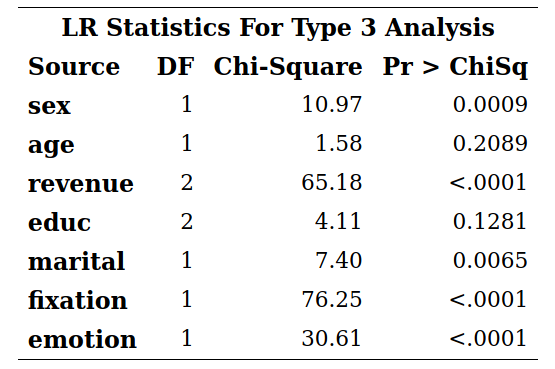
\includegraphics[width = 0.5\linewidth]{img/c4/slides8-e4}
\end{center}
 Five explanatory variables  are statistically significant according to the likelihood ratio tests. 
\end{frame}


\begin{frame}[fragile]
\frametitle{Parameter estimates for Poisson regression}
\begin{center}
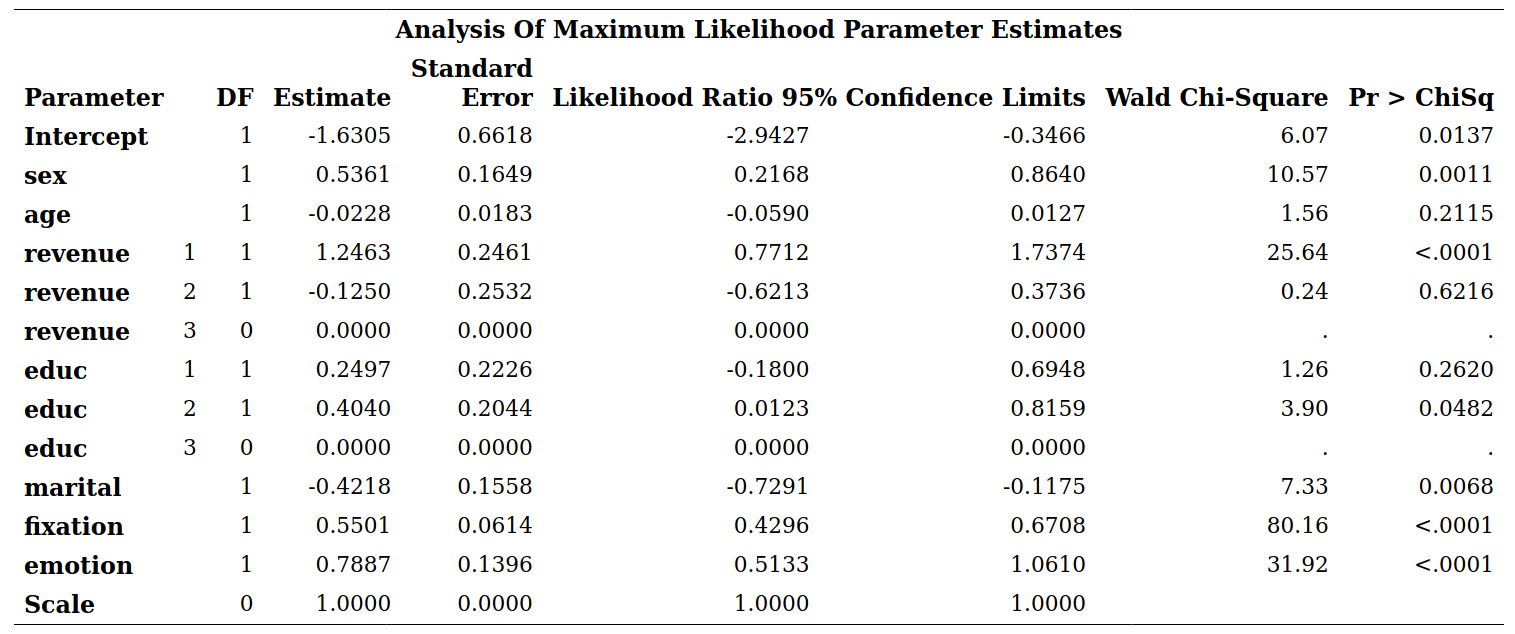
\includegraphics[width = 0.99\linewidth]{img/c4/slides8-e5}
\end{center}
{\footnotesize
The scale parameter is unity because it is completely determined by the mean-variance relationship.

}
\end{frame}

\begin{frame}[fragile]
\frametitle{Interpretation of significant parameters}
\bi
\item The estimate $\hat{\beta}_{\code{sex}}=0.5361$, meaning that \alert{women made more purchases than men, on average}. When the other variables remain constant, the mean number of purchases for women is 
$\exp(0.5361) = 1.71$ times that of men. So, the mean for women is $71$\% higher than for men.
\item The parameter estimate for \texttt{fixation} is $\hat{\beta}_{\code{fixation}}=0.5501$ and it's significantly different from $0$.
The higher the value of \texttt{fixation}, the higher the number of purchases, on average. When the other variables remain constant, increasing
\texttt{fixation} by one unit means the mean number of purchases is multiplied by $\exp(0.5501) =
1.73$.
\item \textit{Ceteris paribus}, the average number of items bought by people with low revenue is $3.47$ higher than those with high income, a relative mean increase of $247$\%.
\ei
\end{frame}
\begin{frame}
 \frametitle{Goodness of fit}
 {\small 
\bi \item  The SAS output includes a table containing the log-likelihood (full log-likelihood) and information criteria. 
\item For the Poisson regression model, the deviance and Pearson $X^2$ statistics are two goodness-of-fit indicators used to determine if the model is adequate.\ei
}
\begin{center}
 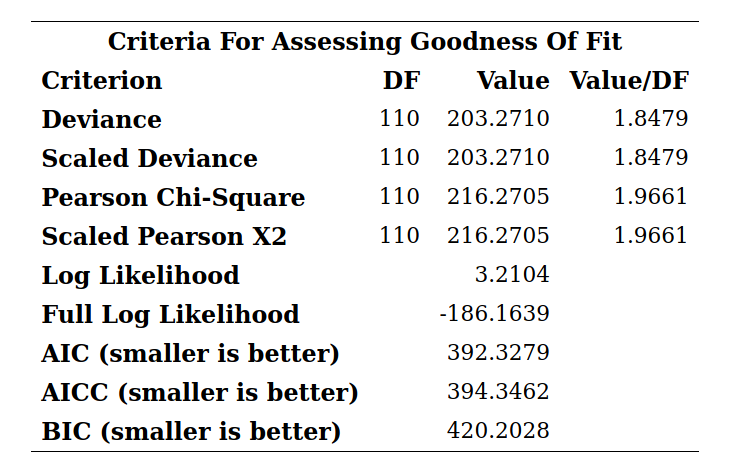
\includegraphics[width = 0.7\linewidth]{img/c4/slides8-e3}
 \end{center}
 {\tiny
 The first two lines are duplicated; the Poisson model has no separate scale parameter, since the variance is fully determined by the mean (unlike linear regression).
 
 }
\end{frame}
\end{document}
